% Provenance (never printed): see sources/outline_sources.md (Year 3: primordial
% nucleosynthesis and stellar burning recalled from the physics books; the s and r
% processes; supernovae and neutron-star mergers; galactic chemical evolution; from the
% solar abundances to the composition of the Earth).
% Brief: sources/book5/BRIEFS.md, ch. 30. Curves from figdata/bachelor-3/
% solar_abundances.py (Asplund, Amarsi and Grevesse 2021, Table 2), neutron_capture.py
% (their Table B.1 isotopes, KADoNiS v0.3 cross sections, IAEA Live Chart half-lives) and
% chemical_evolution.py (closed box against the Geneva-Copenhagen survey of Casagrande et
% al. 2011, and a two-phase [alpha/Fe] model). Exercise and problem values in the Book 5
% scratch calculator calc/ch30.py.
\chapter{Where the Elements Come From}\label{ch:b3:origin-of-elements}

The calcium of a limestone cliff was made, for the most part, inside
massive stars that exploded before the Sun was born. The iron of the
Earth's core comes mostly from a different kind of explosion, that of a
white dwarf. The platinum of a ring belongs to a peak of abundance built
by bursts of \omterm{def:b3:origin-of-elements:s-process}{neutron captures} lasting seconds, in mergers of two neutron
stars or in a rare kind of supernova; which of the two made most of it is
still debated.
Each of these events has left its mark in the composition of the Sun,
which is also, apart from the few elements that the planets could not
keep, the composition of the Solar System. This chapter reads that
record: it sets out the \omterm{def:b3:origin-of-elements:abundance}{solar abundances}, recalls how the light elements
were made, follows the \omterm{def:b3:origin-of-elements:s-process}{neutron captures} that built the heavy ones, finds
the sites where each process runs, and models how the composition of a
galaxy changes as its stars live and die. It ends where the geology of
the earlier volumes begins: why the Earth, made of the same material as
the Sun, is so rich in iron and so poor in volatiles.
% ledger: matteucci21:production, cowan21:rprocess, kobayashi20:origins, asplund21:fig1

\begin{recall}
Big Bang nucleosynthesis, the fusion of hydrogen and helium in stars,
the binding energy per nucleon and its maximum near iron, the valley of
stability, beta decay and half-lives, the cross-section of a reaction,
main-sequence stars, red giants, white dwarfs, neutron stars and
supernovae are in the physics books. The meteorite classes, the CI
chondrites, the condensation temperature, refractory and volatile
elements, the Goldschmidt classes and the bulk silicate Earth are in the
Year~2 volume, in its chapters on the formation of the planets and on
the elements in the Earth. The structure of the Galaxy, its thin and
\omterm{def:b3:milky-way-galaxies:structure}{thick discs}, its halo and its \omterm{def:b3:milky-way-galaxies:populations}{stellar populations} are in the previous
chapter.
\end{recall}

\section{The solar abundances}\label{sec:b3:origin-of-elements:solar}

The Sun holds more than \qty{99.85}{\percent} of the mass of the Solar
System, and its outer layers have kept, apart from a few light elements
and a slow settling of heavy ones, the composition of the gas from which
the Sun and the planets formed. Its composition is read in two ways:
from the absorption lines of its photosphere, and from the CI chondrites,
the meteorites whose composition, except for the most volatile
elements, is the closest of all known materials to the Sun's.
% ledger: asplund21:fig1, asplund21:ci

\begin{definition}[Solar abundance; dex]\label{def:b3:origin-of-elements:abundance}
The \emph{solar abundance}\index{solar abundance} of an element $X$ is
the number of its atoms relative to those of hydrogen in the Sun,
written on a logarithmic scale on which hydrogen is set at $12$:
\[
\log\varepsilon(X) = 12 + \log_{10}\frac{N_X}{N_\mathrm{H}} .
\]
A difference of one unit in such a logarithm is called a
\emph{dex}\index{dex}: two abundances that differ by $0.3$~dex differ by
a factor $10^{0.3} \approx 2$. For a star, the abundance relative to the
Sun is written with brackets,
$[X/\mathrm{H}] = \log_{10}(N_X/N_\mathrm{H})_\star -
\log_{10}(N_X/N_\mathrm{H})_\odot$, and likewise $[X/Y]$ for any two
elements.
\end{definition}

The figure below shows the \omterm{def:b3:origin-of-elements:abundance}{solar abundances} of the recent compilation
that reassessed all 83 long-lived elements. Iron, at
$\log\varepsilon = 7.46$, has one atom for every \num{34700} atoms of
hydrogen; helium has \num{0.0820} atoms per hydrogen atom. Several
features stand out, and the rest of the chapter explains them.
% ledger: asplund21:abstract, asplund21:ci, data:b5-asplund21

\begin{omfigure}
\centering
\begin{tikzpicture}
\begin{axis}[width=0.95\linewidth, height=8.4cm, xmin=0, xmax=94,
  ymin=-1.8, ymax=12.8, xlabel={atomic number $Z$},
  ylabel={$\log\varepsilon(X)$ \;($\log\varepsilon(\mathrm{H}) = 12$)},
  tick label style={font=\scriptsize}, label style={font=\small},
  legend style={font=\scriptsize, at={(0.5,-0.17)}, anchor=north,
    legend columns=2, draw=none, cells={anchor=west},
    /tikz/every even column/.append style={column sep=1em}}]
\addplot[blue!70!black, mark=*, mark size=1.3pt, restrict x to domain=0:84]
  table[x=Z, y=logeps] {figdata/out/bachelor-3-solar_abundances-even.dat};
\addlegendentry{even $Z$}
\addplot[blue!70!black, mark=*, mark size=1.3pt, restrict x to domain=88:94, forget plot]
  table[x=Z, y=logeps] {figdata/out/bachelor-3-solar_abundances-even.dat};
\addplot[red!70!black, mark=o, mark size=1.4pt]
  table[x=Z, y=logeps] {figdata/out/bachelor-3-solar_abundances-odd.dat};
\addlegendentry{odd $Z$}
\begin{scope}[font=\scriptsize]
\node[anchor=west] at (axis cs:2.2,12.2) {H};
\node[anchor=west] at (axis cs:3.0,10.9) {He};
\node[anchor=west] at (axis cs:5.6,1.0) {Li, Be, B};
\node[anchor=south] at (axis cs:8,8.95) {O};
\node[anchor=south] at (axis cs:6,8.6) {C};
\node[anchor=south, align=center] at (axis cs:26,7.75) {Fe\\[-1pt]peak};
\node[anchor=north] at (axis cs:21,2.95) {Sc};
\node[anchor=south, align=center] at (axis cs:38.5,3.05) {Sr--Zr\\[-1pt]($N = 50$)};
\node[anchor=south] at (axis cs:51.5,2.5) {Te, Xe (r)};
\node[anchor=south, align=center] at (axis cs:58.5,3.7) {Ba\\[-1pt]($N = 82$)};
\node[anchor=south] at (axis cs:76.5,1.95) {Pt (r)};
\node[anchor=south, align=center] at (axis cs:82.5,2.85) {Pb\\[-1pt]($N = 126$)};
\node[anchor=south] at (axis cs:89.6,0.15) {Th};
\node[anchor=north] at (axis cs:92,-0.7) {U};
\end{scope}
\end{axis}
\end{tikzpicture}
\par\smallskip{\small The abundances of the elements in the Sun, on a
logarithmic scale with hydrogen at 12: photospheric values, or those of
the CI chondrites for the elements that have no measurable photospheric
line (Asplund, Amarsi and Grevesse, 2021). Even and odd atomic numbers
are drawn as two lines. Technetium ($Z = 43$) and promethium ($Z = 61$)
have no long-lived isotope, nor have the elements between bismuth and
thorium.}\label{fig:b3:origin-of-elements:curve}
\end{omfigure}
% ledger: data:b5-asplund21, asplund21:fig1

\begin{enumerate}
\item Hydrogen and helium make almost all the atoms, a thousand times
  more than all the others together; both were made in the Big Bang, and
  some of the helium since then in stars.
\item Lithium, beryllium and boron, just after helium, lie far below
  carbon: beryllium is twelve million times less abundant.
\item The abundances fall steeply from oxygen to the heavy elements, with
  peaks around oxygen, around iron, around barium and around lead, and
  smaller ones that the figure labels.
\item Elements of even atomic number are more abundant than their odd
  neighbours: scandium, between calcium and titanium, is about \num{1400}
  times rarer than calcium and \num{68} times rarer than titanium. This
  is the \emph{odd--even effect}.
\item Beyond the iron peak the curve flattens: from iron to gold the
  abundance drops by a factor of \num{3.5e6}, but from gold to lead it
  rises again, by a factor of eleven.
\end{enumerate}
% ledger: asplund21:fig1, data:b5-asplund21

By mass, the present photosphere is $X = 0.7438$ hydrogen,
$Y = 0.2423$ helium and $Z = 0.0139$ of everything else. Corrected for
the heavy elements that have settled below the photosphere since the Sun
formed, the proto-solar values, those of the gas the Sun was born from,
are $X = 0.7121$, $Y = 0.2725$ and $Z = 0.0154$.
% ledger: asplund21:xyz

\begin{definition}[Metallicity]\label{def:b3:origin-of-elements:metallicity}
The \emph{metallicity}\index{metallicity} of a star or of a gas is its
content of elements heavier than helium, called metals in astronomy
whatever their chemistry: as a mass fraction $Z$, or, as it is usually
measured, as the iron abundance relative to the Sun, $[\mathrm{Fe/H}]$.
A star with $[\mathrm{Fe/H}] = -1$ has a tenth of the Sun's iron per
hydrogen atom.
\end{definition}

The two sources of the \omterm{def:b3:origin-of-elements:abundance}{solar abundances} agree remarkably well. The
figure below compares them element by element. For 58 elements, those
neither too volatile for the meteorites nor destroyed in the Sun, the
weighted mean difference between the photospheric and the CI abundance
is $\num[separate-uncertainty=true]{0.000 \pm 0.007}$~\omterm{def:b3:origin-of-elements:abundance}{dex}. Two groups
fall off the line. The meteorites hold far less hydrogen, helium,
carbon, nitrogen, oxygen and noble gases than the Sun: these elements
stayed in the gas when the solids condensed. The Sun holds
\num{200} times less lithium than the meteorites: it has destroyed
\qty{99.5}{\percent} of its lithium by nuclear burning.
% ledger: asplund21:ci, data:b5-asplund21

\begin{omfigure}
\centering
\begin{tikzpicture}
\begin{axis}[width=0.66\linewidth, height=0.66\linewidth, xmin=-3, xmax=12.8,
  ymin=-1, ymax=12.8, xlabel={$\log\varepsilon$ in the CI chondrites},
  ylabel={$\log\varepsilon$ in the photosphere},
  tick label style={font=\scriptsize}, label style={font=\small},
  scatter/classes={0={mark=*, mark size=1.3pt, black!70},
    1={mark=square*, mark size=1.5pt, red!70!black},
    2={mark=triangle*, mark size=2pt, blue!70!black}}]
\addplot[black!40, dashed, domain=-1:12.8, samples=2] {x};
\addplot[scatter, only marks, scatter src=explicit symbolic]
  table[x=ci, y=phot, meta=group] {figdata/out/bachelor-3-solar_abundances-compare.dat};
\begin{scope}[font=\scriptsize, red!60!black]
\node[anchor=east] at (axis cs:8.12,12.0) {H};
\node[anchor=west] at (axis cs:1.45,10.914) {He};
\node[anchor=east] at (axis cs:7.25,8.55) {C};
\node[anchor=east] at (axis cs:6.1,7.83) {N};
\node[anchor=west] at (axis cs:8.5,8.45) {O};
\node[anchor=west] at (axis cs:-0.97,8.06) {Ne};
\node[anchor=west] at (axis cs:-0.35,6.38) {Ar};
\node[anchor=west] at (axis cs:-2.12,3.12) {Kr};
\node[anchor=west] at (axis cs:-1.8,2.22) {Xe};
\end{scope}
\node[font=\scriptsize, blue!60!black, anchor=west] at (axis cs:3.4,0.96) {Li};
\end{axis}
\end{tikzpicture}
\par\smallskip{\small The Sun against the CI chondrites: each point is
one element with both values (Asplund, Amarsi and Grevesse, 2021; the
meteoritic scale is fixed so that silicon agrees). The dashed line is
equality. Black dots: the 58 elements that agree. Squares: hydrogen,
helium, carbon, nitrogen, oxygen and the noble gases, which the
meteorites did not keep. Triangle: lithium, destroyed in the
Sun.}\label{fig:b3:origin-of-elements:sun-ci}
\end{omfigure}
% ledger: data:b5-asplund21, asplund21:ci

The agreement is a fact of great weight for geology. It means that the
meteorites, which can be analysed in the laboratory, give the composition of the
Solar System for all but the most volatile elements; and that the Sun,
whose photosphere gives hydrogen, carbon, nitrogen and oxygen, fills in
the rest. The Year~2 volume built the composition of the bulk Earth on
that foundation.
% ledger: asplund21:ci

\section{The light elements and the stars}\label{sec:b3:origin-of-elements:stars}

The physics books describe Big Bang nucleosynthesis: in the first three
minutes, as the Universe cooled, protons and neutrons combined into
deuterium, helium-3, helium-4 and a trace of lithium-7, and into nothing
heavier. The observed primordial abundances are a helium mass fraction
$Y_\mathrm{p} = \num[separate-uncertainty=true]{0.245 \pm 0.003}$, a
deuterium-to-hydrogen ratio of \num{2.5e-5} and a lithium-to-hydrogen
ratio of \num{1.45e-10}, the last measured in old metal-poor stars of
the Galactic halo. All the other elements, and the excess of helium in
the Sun, $0.2725 - 0.245 \approx 0.028$, were made in stars.
% ledger: pdg25:bbn, asplund21:xyz

The stars of the physics books burn hydrogen into helium on the main
sequence, then helium into carbon and oxygen as red giants; the most
massive go on, in shells around their cores, to neon, magnesium,
silicon and finally iron. Fusion stops there, because the binding energy
per nucleon is greatest near iron: building heavier nuclei by fusion
absorbs energy instead of releasing it. Beyond the iron peak, the
elements are built by another route, the capture of neutrons, the
subject of the next section. Lithium, beryllium and boron are fragile:
they are destroyed at the temperatures of stellar interiors, which is
why the Sun has burnt nearly all its lithium, and why the three elements
form a trough in the abundance curve.

\begin{definition}[Alpha element]\label{def:b3:origin-of-elements:alpha}
An \emph{alpha element}\index{alpha element} is one of the even-$Z$
elements oxygen, neon, magnesium, silicon, sulfur and calcium, whose
most abundant isotopes ($^{16}\mathrm{O}$, $^{20}\mathrm{Ne}$,
$^{24}\mathrm{Mg}$, $^{28}\mathrm{Si}$, $^{32}\mathrm{S}$,
$^{40}\mathrm{Ca}$) have mass numbers that are multiples of four, and
which are made mainly in massive stars and returned to the gas by their
explosion as core-collapse supernovae.
\end{definition}
% ledger: matteucci21:production, data:b5-asplund21

The peaks of oxygen and of the \omterm{def:b3:origin-of-elements:alpha}{alpha elements}, and the odd--even effect,
are the marks of these burning stages: helium nuclei are built into the
even nuclei more readily than anything into the odd ones, and nuclei
with even numbers of protons are more tightly bound. What a star returns
to the gas depends on its mass.

\begin{definition}[Stellar yield]\label{def:b3:origin-of-elements:yield}
The \emph{stellar yield}\index{stellar yield} of an element from a star
of given initial mass is the mass of that element which the star has
newly made and returns to the interstellar gas, in winds and in its
final explosion, as a fraction of the star's mass.
\end{definition}
% ledger: matteucci21:yield

Stars of less than \qty{0.8}{M_\odot} live longer than the age of the
Universe and return nothing. Stars of \num{0.8} to \qty{8}{M_\odot}
return helium, nitrogen, carbon and the heavy elements of the \omterm{def:b3:origin-of-elements:s-process}{s process}
(barium, yttrium, strontium) in their winds, and end as carbon--oxygen
white dwarfs. Stars of more than \num{8} to \qty{10}{M_\odot} make
mainly the \omterm{def:b3:origin-of-elements:alpha}{alpha elements} and some iron, and explode as core-collapse
supernovae. A white dwarf in a close binary can explode as a Type~Ia
supernova, and such explosions make the bulk of the iron.
% ledger: matteucci21:production

\begin{omfigure}
\centering
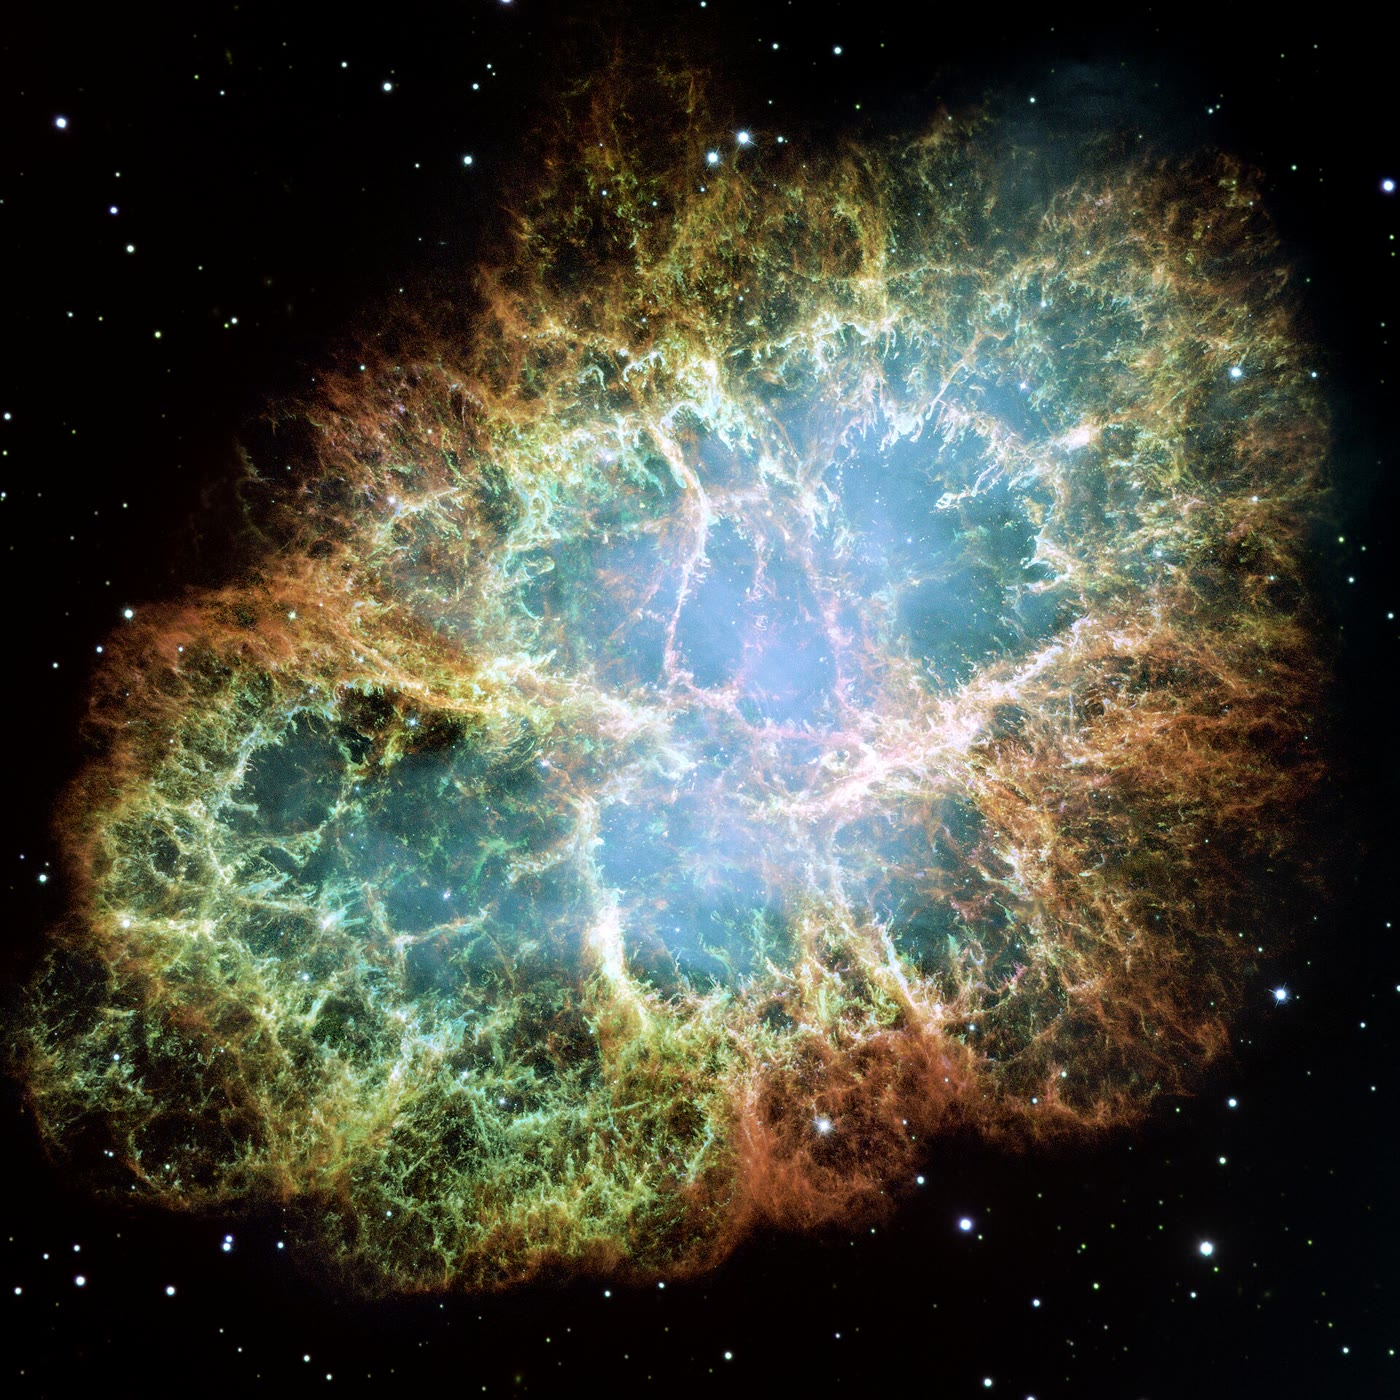
\includegraphics[width=0.5\linewidth]{images/book5/b3-crab-nebula.jpg}
\par\smallskip{\small The Crab Nebula, a mosaic of 24 Hubble Space
Telescope exposures: the expanding remains of a star whose explosion
Japanese and Chinese astronomers recorded in 1054. The orange filaments
are the tattered outer layers of the star, mostly hydrogen; the bluish
glow inside comes from electrons spiralling around the magnetic field
lines of the neutron star at the centre, which spins thirty times a
second. The gas of the filaments, carrying what the star made, mixes
into the interstellar medium. NASA, ESA, J.~Hester and A.~Loll, public
domain.}\label{fig:b3:origin-of-elements:crab}
\end{omfigure}
% ledger: photo:b3-crab-nebula

\section{Neutron captures}\label{sec:b3:origin-of-elements:neutrons}

A neutron has no electric charge and is not repelled by a nucleus: even
a slow neutron enters it, and the nucleus, one mass unit heavier, sheds
the binding energy as a gamma ray. Repeated captures make heavier
isotopes of the same element until one is unstable; it then decays,
usually by beta-minus decay, into the next element, which captures in
turn. Which nuclei are made depends on one comparison: the time between
two captures against the half-life of the unstable nuclei met on the
way.

\begin{definition}[Neutron capture; s process; r process]\label{def:b3:origin-of-elements:s-process}
\emph{Neutron capture}\index{neutron capture} is the absorption of a
free neutron by a nucleus, $(Z, A) + \mathrm{n} \to (Z, A+1) + \gamma$.
In the \emph{s process}\index{s-process@s process} (slow), the captures
are slower than most beta decays: the time between two captures on one
nucleus is hundreds to thousands of years, so an unstable nucleus
nearly always decays before it can capture, and the chain of captures
and decays follows the valley of stability. In the
\emph{r process}\index{r-process@r process} (rapid), the neutron density
is so high that captures are far faster than the decays: the nuclei are
driven to very neutron-rich isotopes, far from stability, in a few
seconds, and decay back to stability once the neutrons run out.
\end{definition}
% ledger: cowan21:timescales, cowan21:rprocess, kaeppeler11:overview

The two processes reach different nuclei, and the chart of the nuclides
shows which. The figure below draws a strip of it, from cadmium to
barium. The \omterm{def:b3:origin-of-elements:s-process}{s process} climbs it along the valley of stability: along a
row of an element while the isotopes are stable, then up one row by a
beta decay. The \omterm{def:b3:origin-of-elements:s-process}{r process} comes from the neutron-rich side, bottom
right: each very neutron-rich nucleus decays by successive beta-minus
decays along its isobar, keeping its mass number, and stops at the first
stable nucleus it meets. A stable nucleus that has a stable isobar of
lower $Z$ is \emph{shielded} from the \omterm{def:b3:origin-of-elements:s-process}{r process}: $^{122}\mathrm{Te}$
lies behind $^{122}\mathrm{Sn}$, $^{123}\mathrm{Te}$ behind
$^{123}\mathrm{Sb}$, $^{124}\mathrm{Te}$ behind $^{124}\mathrm{Sn}$.
Those three can only be made by the \omterm{def:b3:origin-of-elements:s-process}{s process}: they are
\emph{s-only}. Conversely, $^{128}\mathrm{Te}$ and $^{130}\mathrm{Te}$
lie beyond the s path, which leaves tellurium at $^{127}\mathrm{Te}$,
whose half-life is \qty{9.35}{h}: they are r-only.
% ledger: kaeppeler11:overview, data:b5-iaea-gs, data:b5-sigman

\begin{omfigure}
\centering
\begin{tikzpicture}
\begin{axis}[x=0.62cm, y=0.7cm, xmin=61.4, xmax=84.6, ymin=47.4, ymax=56.6,
  xlabel={neutron number $N$}, ylabel={},
  xtick={62,64,...,84}, ytick={48,...,56},
  yticklabels={Cd 48, In 49, Sn 50, Sb 51, Te 52, I 53, Xe 54, Cs 55, Ba 56},
  tick label style={font=\scriptsize}, label style={font=\small},
  axis line style={black!40}, clip=false,
  scatter/classes={0={mark=square*, mark size=6.5pt, blue!45},
    1={mark=square*, mark size=6.5pt, black!18},
    2={mark=square*, mark size=6.5pt, red!40},
    3={mark=square*, mark size=6.5pt, orange!45}}]
\addplot[only marks, mark=square, mark size=6.5pt, black!45, thin,
  restrict x to domain=61:85]
  table[x=N, y=Z] {figdata/out/bachelor-3-neutron_capture-unstable.dat};
\addplot[scatter, only marks, scatter src=explicit symbolic,
  restrict x to domain=61:85]
  table[x=N, y=Z, meta=cls] {figdata/out/bachelor-3-neutron_capture-chart.dat};
\addplot[only marks, mark=none, nodes near coords={\massnum},
  restrict x to domain=61:85,
  visualization depends on={value \thisrow{A} \as \massnum},
  nodes near coords align={center}, every node near coord/.append style={font=\tiny}]
  table[x=N, y=Z] {figdata/out/bachelor-3-neutron_capture-chart.dat};
\addplot[only marks, mark=none, nodes near coords={\massnum}, restrict x to domain=61:85,
  visualization depends on={value \thisrow{A} \as \massnum},
  nodes near coords align={center}, every node near coord/.append style={font=\tiny, black!55}]
  table[x=N, y=Z] {figdata/out/bachelor-3-neutron_capture-unstable.dat};
\addplot[quiver={u=0.48*\thisrow{dN}, v=0.48*\thisrow{dZ}}, -{Stealth[length=3pt]},
  blue!60!black, semithick, restrict x to domain=61:85]
  table[x expr=\thisrow{N0}+0.26*\thisrow{dN}, y expr=\thisrow{Z0}+0.26*\thisrow{dZ}]
  {figdata/out/bachelor-3-neutron_capture-path.dat};
\begin{scope}[red!70!black, dashed, -{Stealth[length=4pt]}, thick]
\draw (axis cs:79.1,48.9) -- (axis cs:76.4,51.6);
\draw (axis cs:81.1,48.9) -- (axis cs:78.4,51.6);
\draw (axis cs:83.1,50.9) -- (axis cs:80.4,53.6);
\end{scope}
\node[font=\scriptsize, red!70!black, anchor=south east, align=right] at (axis cs:84.5,47.5)
  {r-process decays\\[-1pt]along isobars};
\end{axis}
\end{tikzpicture}
\par\smallskip{\small A strip of the chart of the nuclides, from cadmium
to barium, neutron numbers 62 to 84. Coloured squares are the nuclei found in nature, labelled
with their mass number: blue, s-only; grey, made by both processes; red,
r-only; orange, \omterm{def:b3:origin-of-elements:p-process}{p nuclei}, reached by neither. Open squares are the
unstable nuclei the \omterm{def:b3:origin-of-elements:s-process}{s process} passes through. Blue arrows: the s path,
captures to the right, beta decays diagonally up and to the left (at
$^{134}\mathrm{Cs}$ and $^{135}\mathrm{Cs}$ the path splits). Dashed red
arrows: three of the r-process decay chains, ending on
$^{128}\mathrm{Te}$, $^{130}\mathrm{Te}$ and $^{134}\mathrm{Xe}$. The
classes are computed from the isotopes found in nature (Asplund,
Amarsi and Grevesse, 2021) and the half-lives and decay modes of the
IAEA chart of nuclides.}\label{fig:b3:origin-of-elements:chart}
\end{omfigure}
% ledger: data:b5-sigman, data:b5-iaea-gs, data:b5-asplund21, kaeppeler11:branchings

A third group, the orange squares, is reached by neither process: the
proton-rich isotopes such as $^{112}\mathrm{Sn}$, $^{120}\mathrm{Te}$
or $^{124}\mathrm{Xe}$.

\begin{definition}[p nuclei]\label{def:b3:origin-of-elements:p-process}
The \emph{p nuclei}\index{p nuclei} are the stable isotopes on the
proton-rich side of the valley of stability, beyond the iron peak, that
neither the s nor the \omterm{def:b3:origin-of-elements:s-process}{r process} can make: they are shielded from the \omterm{def:b3:origin-of-elements:s-process}{r
process} by a stable isobar of lower $Z$ and lie off the s path. They are
ascribed to a separate p process, probably in supernova explosions, and
with few exceptions their abundances are much smaller than those of the
neighbouring s and r isotopes.
\end{definition}
% ledger: kaeppeler11:overview

The rule that reads the chart, applied to all 287 nuclides of the
proto-solar table beyond zinc, finds 30 s-only nuclei, 29 r-only nuclei
and 36 \omterm{def:b3:origin-of-elements:p-process}{p nuclei}. One of these \omterm{def:b3:origin-of-elements:p-process}{p nuclei}, $^{176}\mathrm{Hf}$, is in fact
reached by the \omterm{def:b3:origin-of-elements:s-process}{s process} through a long-lived excited state of
$^{176}\mathrm{Lu}$ that the simple rule ignores; the other 35 are the \omterm{def:b3:origin-of-elements:p-process}{p
nuclei} of the literature.
% ledger: data:b5-sigman, kaeppeler11:branchings

The \omterm{def:b3:origin-of-elements:s-process}{s process} can be followed quantitatively, because its nuclei are
near stability and their capture cross-sections can be measured. In a
stellar plasma at temperature $T$ the neutrons are thermalised, and what
matters is the cross-section averaged over their Maxwell--Boltzmann
distribution, $\langle\sigma\rangle$, quoted for a thermal energy
$kT = \qty{30}{keV}$.
% ledger: kaeppeler11:classical

\begin{proposition}[The $\sigma N$ relation]\label{prop:b3:origin-of-elements:sigma-n}
\index{sigma N relation@$\sigma N$ relation}
On a stretch of the s path where every nucleus is stable and the neutron
density $n_\mathrm{n}$ and temperature are constant, let $N_A$ be the
abundance of the nucleus of mass number $A$ and $\langle\sigma\rangle_A$
its averaged cross-section. If the neutron flow has reached a steady
state, then
\[
\langle\sigma\rangle_{A-1} N_{A-1} = \langle\sigma\rangle_A N_A ,
\]
so that the product $\sigma N$ is the same for every nucleus of the
stretch.
\end{proposition}

\begin{proof}
A nucleus of mass $A$ captures neutrons at the rate
$\lambda_A = n_\mathrm{n}\langle\sigma\rangle_A v_T$ per nucleus, with
$v_T$ the mean thermal speed of the neutrons. It is made by captures on
$A - 1$ and destroyed by captures on itself, so
$\mathrm{d}N_A/\mathrm{d}t = n_\mathrm{n} v_T\,(\langle\sigma\rangle_{A-1}
N_{A-1} - \langle\sigma\rangle_A N_A)$. In a steady state the derivative
vanishes, which is the relation. A nucleus with a large cross-section is
quickly passed on and stays rare; one with a small cross-section piles
up.
\end{proof}
% ledger: kaeppeler11:classical

The three s-only isotopes of tellurium test it. Their proto-solar
abundances are \num{0.1067}, \num{0.0373} and \num{0.1984} atoms per
million silicon atoms, and their cross-sections \num{295}, \num{832} and
\qty{155}{mb}: the products are \num{31.5}, \num{31.0} and
\qty{30.8}{mb}, equal within three per cent, although the abundances
differ by a factor of five. Across a neutron magic number the relation
breaks: nuclei with $N = 50$, $82$ or $126$ are so tightly bound that
they capture poorly, $\langle\sigma\rangle = \qty{4.0}{mb}$ for
$^{138}\mathrm{Ba}$ against \qty{61.2}{mb} for $^{136}\mathrm{Ba}$, and
they act as bottlenecks. The figure below shows the product for all the
s-only nuclei: flat plateaus separated by steps near $A = 88$, $140$
and $208$.
% ledger: data:b5-sigman, data:b5-kadonis, kaeppeler11:classical

\begin{omfigure}
\centering
\begin{tikzpicture}
\begin{axis}[width=0.95\linewidth, height=7.4cm, xmin=60, xmax=212,
  ymode=log, ymin=1, ymax=5000, xlabel={mass number $A$},
  ylabel={$\langle\sigma\rangle N$ (mb, per $10^6$ Si atoms)},
  tick label style={font=\scriptsize}, label style={font=\small},
  legend style={font=\scriptsize, at={(0.5,-0.17)}, anchor=north,
    legend columns=2, draw=none, cells={anchor=west},
    /tikz/every even column/.append style={column sep=1em}}]
\draw[black!35, dotted, thick] (axis cs:88,1) -- (axis cs:88,5000);
\draw[black!35, dotted, thick] (axis cs:139,1) -- (axis cs:139,5000);
\draw[black!35, dotted, thick] (axis cs:208,1) -- (axis cs:208,5000);
\addplot[blue!70!black, thick, const plot]
  table[x=A, y=sigN_model] {figdata/out/bachelor-3-neutron_capture-fitted.dat};
\addlegendentry{classical model fitted for $A > 90$}
\addplot[only marks, mark=*, mark size=1.7pt, red!70!black]
  table[x=A, y=sigN] {figdata/out/bachelor-3-neutron_capture-sigman.dat};
\addlegendentry{s-only nuclei}
\begin{scope}[font=\scriptsize]
\node[anchor=south west] at (axis cs:88.5,1.1) {$N = 50$};
\node[anchor=south west] at (axis cs:139.5,1.1) {$N = 82$};
\node[anchor=south east] at (axis cs:207.5,1.1) {$N = 126$};
\node[anchor=south] at (axis cs:123,38) {Te};
\node[anchor=south] at (axis cs:135,33) {Ba};
\node[anchor=north] at (axis cs:149,6.6) {Sm};
\node[anchor=west] at (axis cs:177,1.79) {Lu};
\node[anchor=west] at (axis cs:71,2326) {Ge};
\node[anchor=west] at (axis cs:83,428) {Kr};
\end{scope}
\end{axis}
\end{tikzpicture}
\par\smallskip{\small The product of the neutron-capture cross-section
at \qty{30}{keV} (KADoNiS) and the proto-solar abundance (Asplund,
Amarsi and Grevesse, 2021) for the 30 s-only nuclei. Between the magic
neutron numbers (dotted lines) it is nearly constant; at each the flow
is throttled and the product drops. The line is the classical model
of the \omterm{def:b3:origin-of-elements:s-process}{s process} fitted here to the nuclei heavier than $A = 90$. The
lighter ones need a second, weaker component, made in massive
stars.}\label{fig:b3:origin-of-elements:sigma-n}
\end{omfigure}
% ledger: data:b5-sigman, data:b5-kadonis, data:b5-asplund21, kaeppeler11:classical

The line of the figure is the classical model of the \omterm{def:b3:origin-of-elements:s-process}{s process}: a small
fraction $G$ of the iron-56 is exposed to neutrons, with exposures spread
exponentially about a mean $\tau_0$, and the flow is followed nucleus by
nucleus with the measured cross-sections. Its fit to 22 s-only
nuclei heavier than $A = 90$ (leaving out $^{176}\mathrm{Lu}$, which
decays, and $^{187}\mathrm{Os}$, fed by the decay of
$^{187}\mathrm{Re}$) gives $\tau_0 = \qty{0.31}{mb^{-1}}$ and
$G = \qty{0.054}{\percent}$ of the solar iron-56, close to the
\qty{0.04}{\percent} of the detailed analyses, in which each seed
nucleus captures on average about fifteen neutrons. The lightest s-only
nuclei, germanium-70 and selenium-76, lie far above the line: they need
a second, weak component, made in massive stars.
% ledger: data:b5-sigman, kaeppeler11:classical

Where an unstable nucleus on the path lives about as long as the time
between two captures, the flow splits: part of it decays, part captures.
Such \emph{branchings} occur at $^{79}\mathrm{Se}$, $^{85}\mathrm{Kr}$,
$^{134}\mathrm{Cs}$, $^{147}\mathrm{Pm}$ and $^{151}\mathrm{Sm}$, among
others. A branching lets part of the flow bypass a nucleus: of the two
s-only isotopes of samarium, $^{150}\mathrm{Sm}$ receives the whole
flow and $^{148}\mathrm{Sm}$ only the part that went round the
branching at mass 147, and the ratio of their $\sigma N$, \num{0.87},
measures that share. Since the share depends on the neutron density and
the temperature, the branchings are thermometers and densimeters of the
stars where the \omterm{def:b3:origin-of-elements:s-process}{s process} ran.
% ledger: kaeppeler11:branchings, kaeppeler11:pairs, data:b5-sigman

\begin{inthelab}[Measuring a capture cross-section]
To measure the averaged cross-sections that the \omterm{def:b3:origin-of-elements:s-process}{s process} needs,
physicists reproduce a stellar neutron spectrum at an accelerator.
Protons striking a lithium target make neutrons by the reaction
$^{7}\mathrm{Li}(\mathrm{p},\mathrm{n})^{7}\mathrm{Be}$, whose spectrum
mimics a thermal one at $kT = \qty{25}{keV}$, close to the
\qty{23}{keV} of the helium-shell flashes of a red giant. The sample sits
right against the target, in the strongest flux, and after the
irradiation the gamma rays of the newly made radioactive nuclei are
counted: this activation method works with samples of less than a
microgram. Where the product is stable, the neutrons are sent in pulses
and timed over a flight path to give their energy, and a sphere of
barium fluoride crystals around the sample records the gamma-ray
cascade of each capture.
\end{inthelab}
% ledger: kaeppeler11:lab

\begin{history}[Technetium in red giants]
In 1952 P.~W.~Merrill found the lines of technetium in the spectra of
red giants of spectral type S. Technetium has no stable isotope; the one
made by the \omterm{def:b3:origin-of-elements:s-process}{s process}, $^{99}\mathrm{Tc}$, has a half-life of
\num{211000} years, far shorter than the lives these stars
had lived. The technetium had to have been made inside the stars, and
recently. It was the first direct evidence that stars make elements. In
1957 E.~M. and G.~R.~Burbidge, W.~A.~Fowler and F.~Hoyle, and
independently A.~G.~W.~Cameron, formulated the classical model of the
\omterm{def:b3:origin-of-elements:s-process}{s process}.
\end{history}
% ledger: kaeppeler11:overview, data:b5-iaea-gs

The \omterm{def:b3:origin-of-elements:s-process}{r process} leaves its own peaks. Its path runs close to the neutron
drip line, the limit beyond which a nucleus cannot hold another neutron,
and the flow waits at the nuclei with closed neutron shells, $N = 50$, $82$ and
$126$, until they beta-decay. These waiting points pile up material;
after the final decays to stability the piles lie at mass numbers a few
units lower than the s-process peaks of the same magic numbers, which
are made of stable nuclei: near $A = 130$ (tellurium and xenon) and
$A = 195$ (platinum), against $A = 138$ and $208$ for the s peaks of
barium and lead. The abundance curve shows both sets of peaks side by
side. The \omterm{def:b3:origin-of-elements:s-process}{r process} makes about half the heavy elements, the \omterm{def:b3:origin-of-elements:s-process}{s process}
the other half.
% ledger: cowan21:rprocess, kaeppeler11:overview, kaeppeler11:classical

\section{Where the processes run}\label{sec:b3:origin-of-elements:sites}

The main \omterm{def:b3:origin-of-elements:s-process}{s process} runs in red giants of up to about three solar masses, near
the end of their lives, as asymptotic-giant-branch stars. Between flashes
of helium burning in a shell around their cores, a thin layer rich in
carbon-13 forms; at about \qty{9e7}{K} the reaction
$^{13}\mathrm{C}(\alpha,\mathrm{n})^{16}\mathrm{O}$ releases neutrons
for some ten thousand years, at densities of $10^6$ to
\num{e8}\text{ neutrons}\,\unit{cm^{-3}}. During the flashes themselves, above
\qty{2.5e8}{K}, $^{22}\mathrm{Ne}(\alpha,\mathrm{n})^{25}\mathrm{Mg}$
gives a burst of a few years at up to \qty{e10}{cm^{-3}}. The products
are dredged up to the surface, where technetium is seen, and blown away
in the star's wind. The weak \omterm{def:b3:origin-of-elements:s-process}{s process}, which makes the s-only nuclei
lighter than $A = 90$, runs in massive stars during their helium and
carbon burning.
% ledger: kaeppeler11:sources, kaeppeler11:overview

Core-collapse supernovae, the end of stars above eight to ten solar
masses, return the \omterm{def:b3:origin-of-elements:alpha}{alpha elements} and part of the iron soon after the
stars' birth, because massive stars live short lives. Type~Ia
supernovae, white dwarfs that explode in binaries, return most of the
iron, but only after a delay: the white dwarf must form first, from a
star of less than eight solar masses, and then either gather matter from
a companion until it reaches the Chandrasekhar mass, about
\qty{1.44}{M_\odot}, or merge with a second white dwarf. The \omterm{def:b3:origin-of-elements:s-process}{r process} needs a far more extreme
place.
% ledger: matteucci21:production, matteucci21:time-delay

\begin{definition}[Neutron-star merger; kilonova]\label{def:b3:origin-of-elements:kilonova}
A \emph{neutron-star merger}\index{neutron-star merger} is the
coalescence of two neutron stars in a close binary, whose orbit has
shrunk by the emission of gravitational waves. Part of the neutron-rich
matter is flung out. A \emph{kilonova}\index{kilonova} is the transient
glow of that ejecta, heated by the radioactive decay of the freshly made
r-process nuclei, which lasts for days.
\end{definition}
% ledger: cowan21:kilonova, ligo17:gw170817

On 17 August 2017 the gravitational-wave detectors recorded the
inspiral of two neutron stars, GW170817, at a distance of about
\qty{40}{Mpc}: two bodies of \num{1.17} to \qty{1.60}{M_\odot}, together
\qty{2.74}{M_\odot}. A gamma-ray burst arrived \qty{1.7}{s} after the
merger. Less than eleven hours later telescopes found a new point of
light in the galaxy NGC~4993 (figure below). Its ultraviolet glow faded
within two days, and over ten days its light turned red and infrared.
The models of that evolution need several components of ejecta, the
reddest rich in the lanthanides, heavy r-process elements whose dense
forest of lines makes the ejecta opaque. The total ejected mass is
estimated at \num{0.03} to \qty{0.08}{M_\odot}: the first direct
evidence that \omterm{def:b3:origin-of-elements:kilonova}{neutron-star mergers} make r-process elements.
% ledger: ligo17:gw170817, mma17:kilonova, cowan21:kilonova

\begin{omfigure}
\centering
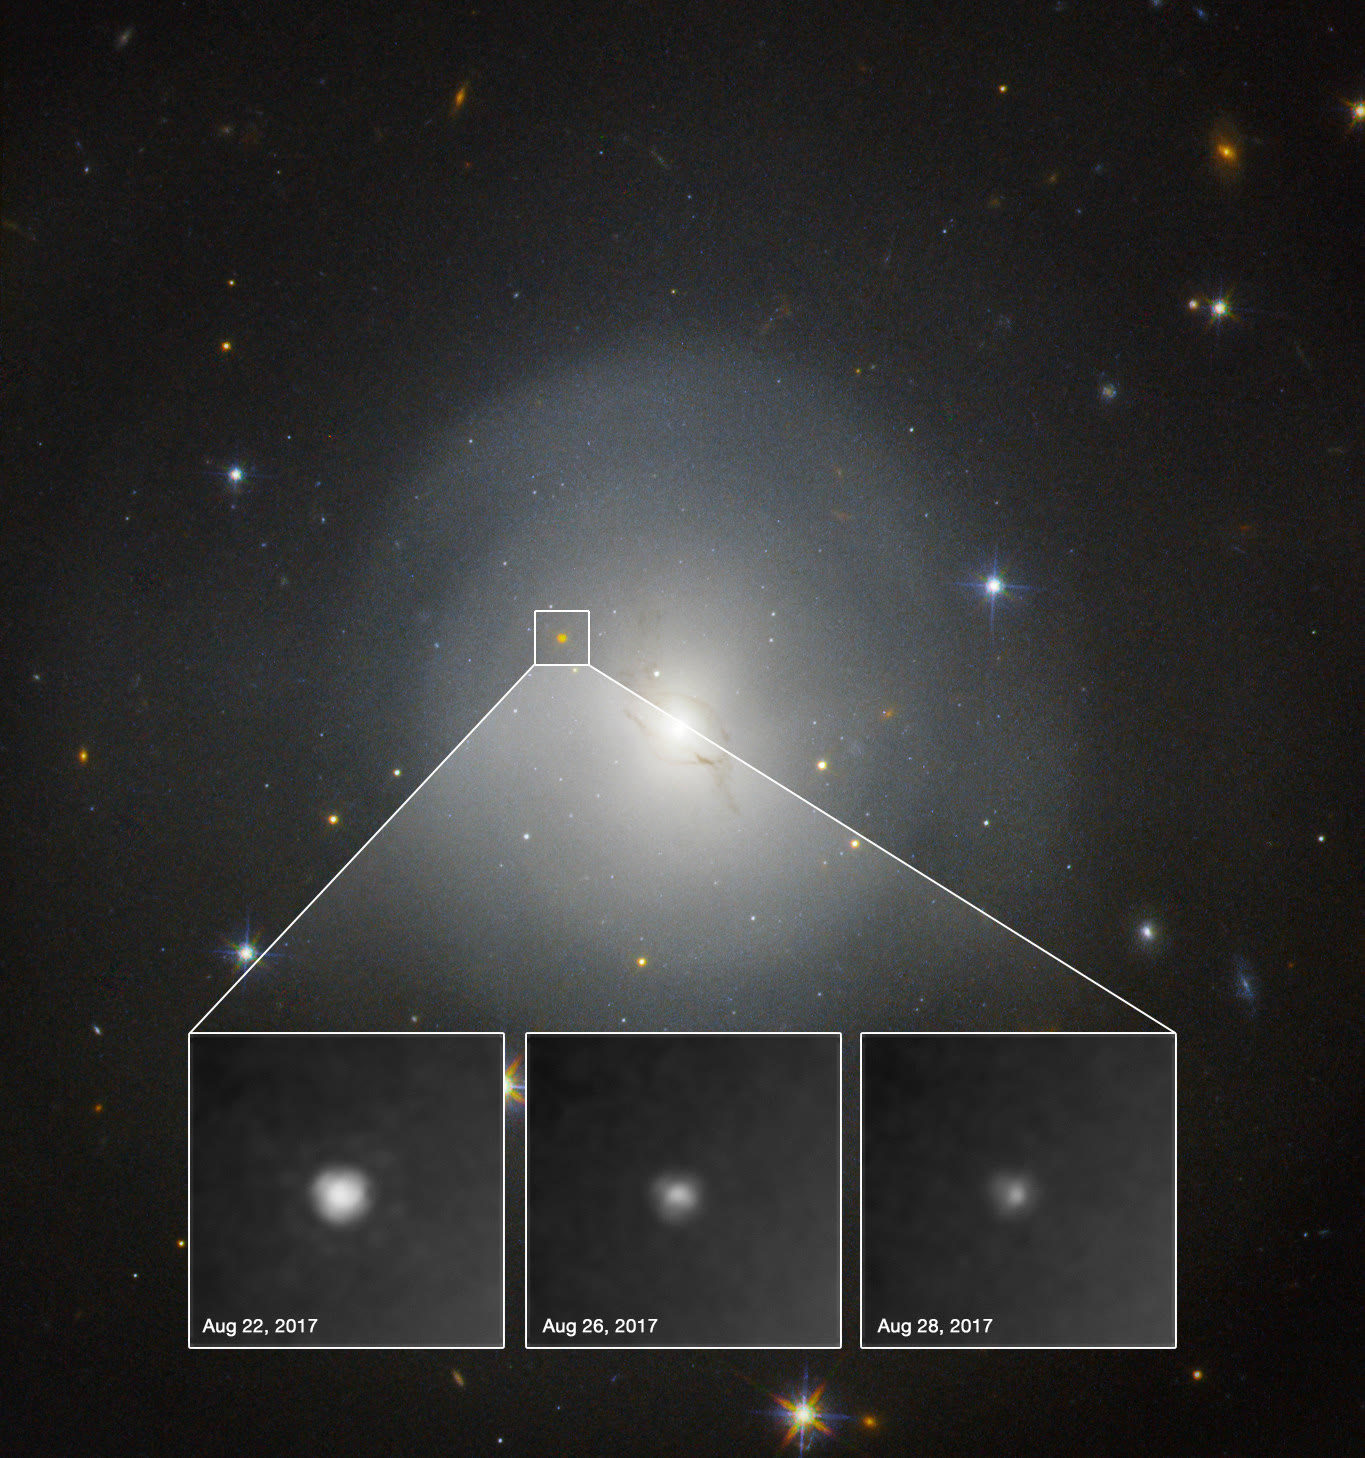
\includegraphics[width=0.55\linewidth]{images/book5/b3-kilonova.jpg}
\par\smallskip{\small The galaxy NGC~4993 photographed by the Hubble
Space Telescope after the merger of two neutron stars detected in
gravitational waves on 17 August 2017. The box marks the \omterm{def:b3:origin-of-elements:kilonova}{kilonova}; the
insets, taken on 22, 26 and 28 August, show it fading over six days.
NASA and ESA (A.~J.~Levan, N.~R.~Tanvir, A.~Fruchter and O.~Fox), CC
BY~4.0.}\label{fig:b3:origin-of-elements:kilonova}
\end{omfigure}
% ledger: photo:b3-kilonova

\begin{dated}{2021}
Whether \omterm{def:b3:origin-of-elements:kilonova}{neutron-star mergers} make most of the Galaxy's r-process
elements is not settled. Mergers wait for their binary orbits to decay,
and models of the Galaxy's evolution in which they are the only source
make the r-process elements too late to explain what is seen in the
oldest, most metal-poor stars. Rare kinds of core-collapse supernova,
with fast rotation and strong magnetic fields, and the collapse of very
massive stars are the other candidates; one model of the Galaxy
explains the observed europium if about three per cent of the
hypernovae of 25 to \qty{50}{M_\odot} are of the magnetically driven
kind.
\end{dated}
% ledger: kobayashi20:origins, cowan21:rprocess

\section{The chemical evolution of the Galaxy}\label{sec:b3:origin-of-elements:gce}

Each generation of stars returns to the gas some of what it made, and
the next generation forms from that enriched gas. The composition of a
star therefore records the composition of the gas at its birth, and the
stars of a galaxy, sorted by age, record its history.

\begin{definition}[Galactic chemical evolution]\label{def:b3:origin-of-elements:gce}
\emph{Galactic chemical evolution}\index{galactic chemical evolution}
is the change of the composition of the gas and of the stars of a
galaxy with time, under the combined action of star formation, the
\omterm{def:b3:origin-of-elements:yield}{stellar yields}, the lifetimes of the stars, and the gas that flows into
the galaxy or is driven out of it; and the study of that change by
models compared with the abundances of stars of known age.
\end{definition}
% ledger: matteucci21:simple

The simplest model treats a region of a galaxy as one well-mixed box of
gas that turns slowly into stars. Let $s$ be the mass locked in
long-lived stars and in stellar remnants, $M_\mathrm{g}$ the mass of
gas, and $M = M_\mathrm{g} + s$ the total. The \emph{yield per stellar
generation} $y$ is the mass of new metals that a generation of stars
returns to the gas per unit mass it locks up.
% ledger: matteucci21:yield

\begin{theorem}[Closed-box model]\label{thm:b3:origin-of-elements:closed-box}
\index{closed-box model}
Consider a region that exchanges no gas with its surroundings, starts as
pure gas without metals, stays well mixed, and in which the stars that
make metals die at once while the others live for ever (instantaneous
recycling). Then the \omterm{def:b3:origin-of-elements:metallicity}{metallicity} of the gas is
\[
Z = y \ln\frac{1}{\mu}, \qquad \mu = \frac{M_\mathrm{g}}{M},
\]
where $\mu$ is the gas fraction, and the mass of stars formed with a
\omterm{def:b3:origin-of-elements:metallicity}{metallicity} below $Z$ is \mbox{$M\,(1 - \mathrm{e}^{-Z/y})$}.
\end{theorem}

\begin{proof}
When a mass $\mathrm{d}s$ is locked into stars, the gas loses
$\mathrm{d}s$, together with the metals it contains, $Z\,\mathrm{d}s$,
and gains $y\,\mathrm{d}s$ of new metals:
$\mathrm{d}M_\mathrm{g} = -\mathrm{d}s$ and
$\mathrm{d}(Z M_\mathrm{g}) = (y - Z)\,\mathrm{d}s$. Expanding the
second, $M_\mathrm{g}\,\mathrm{d}Z + Z\,\mathrm{d}M_\mathrm{g} =
y\,\mathrm{d}s - Z\,\mathrm{d}s$, and the terms in $Z$ cancel:
$M_\mathrm{g}\,\mathrm{d}Z = -y\,\mathrm{d}M_\mathrm{g}$. Integrating
from $M_\mathrm{g} = M$, $Z = 0$ gives $Z = y\ln(M/M_\mathrm{g})$. The
stars formed while the gas \omterm{def:b3:origin-of-elements:metallicity}{metallicity} was below $Z$ are those formed
while the gas fell from $M$ to $M\mathrm{e}^{-Z/y}$, a mass
$M(1 - \mathrm{e}^{-Z/y})$.
\end{proof}
% ledger: matteucci21:simple

The model predicts the \omterm{def:b3:origin-of-elements:metallicity}{metallicity} distribution of the long-lived stars.
In the solar neighbourhood the surface density of gas is
\qty{13.7}{M_\odot.pc^{-2}} and that of stars and stellar remnants
\qty{33.4}{M_\odot.pc^{-2}}, so $\mu = 13.7/47.1 = 0.29$. If the gas
today has the proto-solar $Z = 0.0154$, the yield is
$y = 0.0154/\ln(1/0.29) = 0.0125$, and the fraction of all the stars
formed so far that have $Z$ below a tenth of the present value,
$[\mathrm{Fe/H}] < -1$ if iron follows the metals, is
$(1 - 0.29^{0.1})/(1 - 0.29) = 0.16$.
% ledger: mckee15:surface, asplund21:xyz, data:b5-gce

\begin{omfigure}
\centering
\begin{tikzpicture}
\begin{axis}[width=0.95\linewidth, height=7.2cm, xmin=-1.6, xmax=0.7,
  ymin=0, ymax=1500, xlabel={$[\mathrm{Fe/H}]$},
  ylabel={number of stars per \num{0.1}~dex},
  tick label style={font=\scriptsize}, label style={font=\small},
  legend style={font=\scriptsize, at={(0.5,-0.17)}, anchor=north,
    legend columns=3, draw=none, cells={anchor=west},
    /tikz/every even column/.append style={column sep=1em}}]
\addplot[ybar, area legend, bar width=0.085, fill=black!25, draw=black!50, bar shift=0pt]
  table[x=feh, y=n_obs] {figdata/out/bachelor-3-chemical_evolution-mdf.dat};
\addlegendentry{F and G dwarfs (6670)}
\addplot[ybar, area legend, bar width=0.085, fill=blue!55, draw=blue!70!black, bar shift=0pt]
  table[x=feh, y=n_low] {figdata/out/bachelor-3-chemical_evolution-mdf.dat};
\addlegendentry{at most \qty{1}{M_\odot} (902)}
\addplot[red!75!black, very thick, const plot mark mid]
  table[x=feh, y=model] {figdata/out/bachelor-3-chemical_evolution-mdf.dat};
\addlegendentry{closed box}
\draw[black!50, dashed] (axis cs:-1,0) -- (axis cs:-1,1500);
\node[font=\scriptsize, anchor=north west, align=left] at (axis cs:-1.57,1450)
  {closed box: \qty{16}{\percent}\\below $-1$;\\observed: \qty{0.4}{\percent}};
\end{axis}
\end{tikzpicture}
\par\smallskip{\small The \omterm{def:b3:origin-of-elements:g-dwarf}{G-dwarf problem}. Bars: the metallicities of
the F and G dwarfs of the solar neighbourhood (Geneva--Copenhagen
survey, best-photometry sample re-analysed by Casagrande and others,
2011), all stars in grey, those of at most one solar mass, the long-lived
stars that the model counts, in blue. Line: the closed
box with the present gas fraction of the solar neighbourhood, scaled to
the same number of stars; it makes no star richer than its present gas,
taken as solar. The box predicts a long tail of metal-poor
stars that is not there.}\label{fig:b3:origin-of-elements:g-dwarf}
\end{omfigure}
% ledger: data:b5-gcs, casagrande11:gcs, data:b5-gce, mckee15:surface

\begin{definition}[G-dwarf problem]\label{def:b3:origin-of-elements:g-dwarf}
The \emph{G-dwarf problem}\index{G-dwarf problem} is the shortage of
metal-poor long-lived stars in the solar neighbourhood compared with the
prediction of the \omterm{thm:b3:origin-of-elements:closed-box}{closed-box model}: far fewer of the long-lived dwarf
stars of spectral type G have low metallicities than a closed box would
have made.
\end{definition}
% ledger: matteucci21:simple

Of the 6670 stars of the survey sample, 26 have $[\mathrm{Fe/H}] < -1$:
\qty{0.4}{\percent}, against the \qty{16}{\percent} of the closed box.
Even among the 902 stars of at most a solar mass, the fairest
comparison, the 26 make \qty{2.9}{\percent}. The way out is to open the
box: if the disc of the solar neighbourhood was built by a slow infall
of metal-poor gas over several billion years, the early gas was never
a large reservoir waiting to make metal-poor stars, and the tail
disappears. Models of the disc that reproduce the distribution need an
infall time longer than three to four billion years.
% ledger: data:b5-gcs, data:b5-gce, matteucci21:simple

The second clock is the ratio of two kinds of element. The \omterm{def:b3:origin-of-elements:alpha}{alpha
elements} come from core-collapse supernovae, soon after a stellar
generation is born; much of the iron comes from Type~Ia supernovae,
long after. In old halo stars, with $[\mathrm{Fe/H}] < -1$,
$[\alpha/\mathrm{Fe}]$ is about $+0.4$: these stars formed from gas
enriched by core-collapse supernovae alone. In disc stars it falls with
increasing \omterm{def:b3:origin-of-elements:metallicity}{metallicity} to zero, the solar value, as the Type~Ia
supernovae add their iron. The figure below shows the simplest model
of this \emph{time-delay} picture: in a closed box, both kinds of
supernova start at once except that the Type~Ia start a fixed delay
after the first stars.
% ledger: matteucci21:time-delay, matteucci21:production

\begin{omfigure}
\centering
\begin{tikzpicture}
\begin{axis}[width=0.8\linewidth, height=6.4cm, xmin=-2.4, xmax=0.25,
  ymin=-0.08, ymax=0.55, xlabel={$[\mathrm{Fe/H}]$},
  ylabel={$[\alpha/\mathrm{Fe}]$},
  tick label style={font=\scriptsize}, label style={font=\small}]
\addplot[black!40, dashed, domain=-2.4:0.25, samples=2] {0};
\addplot[blue!70!black, very thick]
  table[x=feh, y=afe] {figdata/out/bachelor-3-chemical_evolution-alpha.dat};
\addplot[only marks, mark=*, mark size=2pt, red!70!black] coordinates {(-1,0.4) (0,0)};
\node[font=\scriptsize, anchor=south, align=center] at (axis cs:-1.75,0.41)
  {core-collapse supernovae only};
\node[font=\scriptsize, anchor=south west, align=left] at (axis cs:-0.98,0.41)
  {Type Ia supernovae\\[-1pt]begin};
\node[font=\scriptsize, anchor=south west] at (axis cs:0.01,0.01) {Sun};
\end{axis}
\end{tikzpicture}
\par\smallskip{\small A two-phase model of $[\alpha/\mathrm{Fe}]$ in a
closed box: the plateau at $+0.4$ is the ratio made by core-collapse
supernovae; Type~Ia supernovae, which begin when the gas has reached
$[\mathrm{Fe/H}] = -1$, then add iron at a steady rate, until the ratio
is solar at $[\mathrm{Fe/H}] = 0$. The plateau and the knee are those
seen in the stars of the Galaxy; the shape between is the model's.
At the Sun's \omterm{def:b3:origin-of-elements:metallicity}{metallicity}, \qty{60}{\percent} of the iron in this model
has come from Type~Ia supernovae.}\label{fig:b3:origin-of-elements:alpha}
\end{omfigure}
% ledger: data:b5-gce, matteucci21:time-delay

The detailed models of the Galaxy that reproduce the observed trend
take two-thirds of the iron from Type~Ia supernovae and one third from
core-collapse supernovae, and find that the gas of the young Galaxy
reached $[\mathrm{Fe/H}] = -1$ in about one to one and a half billion
years. The ratio is a clock: a population that is rich in \omterm{def:b3:origin-of-elements:alpha}{alpha
elements} at a given \omterm{def:b3:origin-of-elements:metallicity}{metallicity} formed its stars fast, before the
Type~Ia supernovae could add their iron. The \omterm{def:b3:milky-way-galaxies:structure}{thick disc} of the previous
chapter is such a population: old, and mildly enriched in \omterm{def:b3:origin-of-elements:alpha}{alpha
elements} compared with thin-disc stars of the same \omterm{def:b3:origin-of-elements:metallicity}{metallicity}.
% ledger: matteucci21:time-delay, casagrande11:gcs

\section{From the solar abundances to the Earth}\label{sec:b3:origin-of-elements:earth}

The Earth is made of the same material as the Sun, but not of all of
it. In the cooling nebula, only the elements that condensed into solids
could be gathered into planetesimals; the Year~2 volume followed the
sequence in which they condense. Iron condenses as metal at about the
same temperature as the magnesium silicates, \qtyrange{1310}{1340}{K} at
\qty{e-4}{bar}, so the rocky planets kept their share of iron, while
hydrogen, helium, carbon, nitrogen and the noble gases stayed in the gas.
Of a gas of solar composition, only about half a per cent of the mass
condenses as rock and metal.
% ledger: lodders:tc-table, lodders:condensates

\begin{definition}[Volatility trend]\label{def:b3:origin-of-elements:volatility}
The \emph{volatility trend}\index{volatility trend} of a planetary body
is the decrease of its abundances, relative to the CI chondrites and
normalised to a refractory element, with decreasing condensation
temperature: refractory elements stand in their chondritic proportions,
moderately volatile ones are depleted the more the lower their
condensation temperature.
\end{definition}

For the silicate Earth, the Year~2 volume drew the trend against the
condensation temperature. Normalised to magnesium, zirconium
(condensing at \qty{1741}{K}) stands at \num{1.11} times its CI
proportion, sodium (\qty{958}{K}) at \num{0.22}, potassium
(\qty{1006}{K}) at \num{0.19}, rubidium (\qty{800}{K}) at \num{0.12}
and zinc (\qty{726}{K}) at \num{0.075}. The Earth formed from material
that had already lost part of its moderately volatile elements before
the planet was assembled, or lost them during its growth. Even the CI
chondrites differ from the Sun in a way that follows the condensation
temperature, though faintly: their moderately volatile elements stand
about \num{0.04}~\omterm{def:b3:origin-of-elements:abundance}{dex} higher than the photospheric values.
% ledger: lodders:tc-table, lodders:ci-table, ms95:pm-trace, asplund21:abstract

So the record of this chapter runs through the planet. The oxygen,
magnesium and silicon of the mantle are \omterm{def:b3:origin-of-elements:alpha}{alpha elements} from massive
stars; the iron of the core came mostly from Type~Ia supernovae; the
thorium and uranium whose decay helps to heat the interior lie beyond
bismuth, where only the \omterm{def:b3:origin-of-elements:s-process}{r process} reaches; and the whole mixture was
sorted by volatility before the Earth gathered it.
% ledger: matteucci21:production, matteucci21:time-delay, kaeppeler11:overview, data:b5-sigman

\section{Exercises}

\begin{exercise}[$\star$]\label{exo:b3:origin-of-elements:1}
Using the \omterm{def:b3:origin-of-elements:abundance}{solar abundances} $\log\varepsilon(\mathrm{O}) = 8.69$,
$\log\varepsilon(\mathrm{Si}) = 7.51$, $\log\varepsilon(\mathrm{Fe}) =
7.46$, $\log\varepsilon(\mathrm{Au}) = 0.91$ and
$\log\varepsilon(\mathrm{Pb}) = 1.95$: (a)~how many silicon atoms and
how many oxygen atoms are there in the Sun per iron atom? (b)~How many
iron atoms per gold atom, and how many lead atoms per gold atom?
\end{exercise}

\begin{exercise}[$\star$]\label{exo:b3:origin-of-elements:2}
(a)~How many iron atoms per million hydrogen atoms does the Sun hold
($\log\varepsilon(\mathrm{Fe}) = 7.46$)? (b)~A halo star has
$[\mathrm{Fe/H}] = -2$. How many hydrogen atoms does it hold per iron
atom? (c)~Another star has one iron atom for every ten million hydrogen
atoms. What is its $[\mathrm{Fe/H}]$?
\end{exercise}

\begin{exercise}[$\star$]\label{exo:b3:origin-of-elements:3}
The stable isotopes of xenon have mass numbers 124, 126, 128, 129, 130,
131, 132, 134 and 136. Among their isobars, tellurium ($Z = 52$) has
stable isotopes 120, 122--126, 128 and 130; iodine ($Z = 53$) only 127.
The s path reaches xenon at $^{128}\mathrm{Xe}$, by the decay of
$^{128}\mathrm{I}$, and leaves it at $^{133}\mathrm{Xe}$, which decays.
Classify each xenon isotope as s-only, r-only, made by both, or p
nucleus.
\end{exercise}

\begin{exercise}[$\star$]\label{exo:b3:origin-of-elements:4}
GW170817 lay at about \qty{40}{Mpc}, and its gamma rays arrived
\qty{1.7}{s} after the merger seen in gravitational waves. (a)~How long
had both signals travelled? (b)~If the delay is set entirely to a
difference in the two speeds, how large is that difference as a
fraction of the speed of light, at most?
\end{exercise}

\begin{exercise}[$\star\star$]\label{exo:b3:origin-of-elements:5}
The three s-only isotopes of tellurium have proto-solar abundances
\num{0.1067}, \num{0.0373} and \num{0.1984} per $10^6$ silicon atoms
($A = 122$, $123$, $124$) and averaged cross-sections \num{295},
\num{832} and \qty{155}{mb}. (a)~Compute $\sigma N$ for each. (b)~From
$^{122}\mathrm{Te}$ alone, predict the abundances of $^{123}\mathrm{Te}$
and $^{124}\mathrm{Te}$, and compare. (c)~Why can the relation not be
applied to $^{128}\mathrm{Te}$?
\end{exercise}

\begin{exercise}[$\star\star$]\label{exo:b3:origin-of-elements:6}
In the classical model, each nucleus on the s path passes on to the
next a fraction $f = 1/(1 + 1/(\tau_0\langle\sigma\rangle))$ of the
flow, with $\tau_0 = \qty{0.306}{mb^{-1}}$. (a)~Compute $f$ for
$^{124}\mathrm{Te}$ (\qty{155}{mb}) and for the neutron-magic
$^{138}\mathrm{Ba}$ (\qty{4.0}{mb}). (b)~The nuclei from
$^{137}\mathrm{Ba}$ to $^{142}\mathrm{Nd}$ on the path have
cross-sections \num{76.3}, \num{4.0}, \num{32.4}, \num{11.0},
\num{111.4} and \qty{35.0}{mb}. By what factor does $\sigma N$ fall from
$^{136}\mathrm{Ba}$ to $^{142}\mathrm{Nd}$? (c)~Compare with the
measured values, \num{27.6} and \qty{7.72}{mb}.
\end{exercise}

\begin{exercise}[$\star\star$]\label{exo:b3:origin-of-elements:7}
A neutron of thermal energy $kT$ has the speed
$v_T = \sqrt{2kT/m_\mathrm{n}}$, $m_\mathrm{n} = \qty{1.6749e-27}{kg}$.
(a)~Compute $v_T$ at $kT = \qty{8}{keV}$, the temperature of the
carbon-13 layer of a red giant. (b)~For $^{124}\mathrm{Te}$, with
$\langle\sigma\rangle = \qty{155}{mb}$, compute the mean time between
two captures, $1/(n_\mathrm{n}\langle\sigma\rangle v_T)$, for
$n_\mathrm{n} = 10^6$, $10^8$ and \qty{e10}{cm^{-3}}. (c)~Compare with
the half-lives of $^{127}\mathrm{Te}$ (\qty{9.35}{h}) and of
$^{134}\mathrm{Cs}$ (\qty{2.07}{yr}). Which one is a branching point?
\end{exercise}

\begin{exercise}[$\star\star$]\label{exo:b3:origin-of-elements:8}
In the Sun, $\log\varepsilon$ is \num{6.30} for calcium, \num{3.14} for
scandium and \num{4.97} for titanium; \num{1.38} for beryllium,
\num{2.70} for boron and \num{8.46} for carbon. (a)~How many times
rarer is scandium than its two neighbours? (b)~How many times rarer is
beryllium than carbon? (c)~Which feature of the abundance curve does
each illustrate, and what is its cause?
\end{exercise}

\begin{exercise}[$\star\star$]\label{exo:b3:origin-of-elements:9}
In the two-phase model of the chapter, the plateau
$[\alpha/\mathrm{Fe}] = P$ is the ratio made by core-collapse supernovae,
and at $[\mathrm{Fe/H}] = 0$ the ratio is solar. (a)~Show that the share
of the solar iron made by Type~Ia supernovae is $1 - 10^{-P}$, and
compute it for $P = 0.4$. (b)~What plateau would give the two-thirds of
the detailed models? (c)~A dwarf galaxy shows its knee at
$[\mathrm{Fe/H}] = -2$. What does that say about its star formation?
\end{exercise}

\begin{exercise}[$\star\star\star$]\label{exo:b3:origin-of-elements:10}
The CI chondrites contain, in parts per million by mass, \num{95870}
of magnesium, \num{3.96} of zirconium, \num{5010} of sodium, \num{530}
of potassium and \num{2.13} of rubidium; the silicate Earth contains
\qty{22.8}{\percent} of magnesium and \num{10.5}, \num{2670}, \num{240}
and \num{0.6} parts per million of the others. Their 50~per~cent
condensation temperatures are \qty{1336}{K} (Mg), \qty{1741}{K} (Zr),
\qty{958}{K} (Na), \qty{1006}{K} (K) and \qty{800}{K} (Rb). (a)~For
each element compute $(X/\mathrm{Mg})_\mathrm{Earth}/(X/\mathrm{Mg})_\mathrm{CI}$.
(b)~Plot it against the condensation temperature and describe the
trend. (c)~Why is magnesium chosen as the reference?
\end{exercise}

\begin{exercise}[$\star\star\star$]\label{exo:b3:origin-of-elements:11}
A leaky box loses gas in a wind at a rate $\lambda$ times its rate of
star formation, and receives none. (a)~Show that its \omterm{def:b3:origin-of-elements:metallicity}{metallicity} is
$Z = \frac{y}{1 + \lambda}\ln\frac{M_\mathrm{g}(0)}{M_\mathrm{g}}$.
(b)~With $y = 0.0125$, compare the \omterm{def:b3:origin-of-elements:metallicity}{metallicity} reached when the gas has
fallen to \qty{29}{\percent} of its initial mass for $\lambda = 0$ and
$\lambda = 1$. (c)~Why do small galaxies, with weak gravity, tend to be
metal-poor?
\end{exercise}

\begin{exercise}[$\star\star\star$]\label{exo:b3:origin-of-elements:12}
(a)~The Sun has $\log\varepsilon(\mathrm{Li}) = 0.96$ in its photosphere
and the CI chondrites $3.25$. Compute the two ratios $N_\mathrm{Li}/N_\mathrm{H}$
and the fraction of its lithium the Sun has destroyed. (b)~The oldest
metal-poor stars show $N_\mathrm{Li}/N_\mathrm{H} = \num{1.45e-10}$,
while Big Bang nucleosynthesis predicts \num{4.72e-10}. By what factor
does the Solar System's lithium exceed each? (c)~What do the two
comparisons imply?
\end{exercise}

\section{Problem: A closed-box galaxy}

\begin{problem}[{Weekend problem --- from the solar mixture to the
metallicities of the long-lived stars}]
\label{pb:b3:origin-of-elements:1}
Use $\log\varepsilon(\mathrm{H}) = 12$, the \omterm{def:b3:origin-of-elements:abundance}{solar abundances}
$\log\varepsilon(\mathrm{Fe}) = 7.46$, $\log\varepsilon(\mathrm{O}) =
8.69$, $\log\varepsilon(\mathrm{He}) = 10.914$, the present
photospheric mass fractions $X = 0.7438$, $Y = 0.2423$, $Z = 0.0139$,
and the proto-solar $Z_\odot = 0.0154$. Assume throughout that iron
follows the total \omterm{def:b3:origin-of-elements:metallicity}{metallicity}, $[\mathrm{Fe/H}] = \log_{10}(Z/Z_\odot)$.

\medskip\noindent\textbf{Part I --- The solar mixture.}
\begin{enumerate}
\item How many hydrogen atoms are there in the Sun per iron atom?
\item Compute the number ratio $N_\mathrm{He}/N_\mathrm{H}$. Taking a
  helium atom four times as heavy as a hydrogen atom, compare
  $4N_\mathrm{He}/N_\mathrm{H}$ with $Y/X$.
\item A star holds one iron atom for every \num{350000} hydrogen atoms.
  Compute its $[\mathrm{Fe/H}]$ to two decimals.
\item The same star has $[\mathrm{O/Fe}] = +0.40$. Compute its
  $\log\varepsilon(\mathrm{O})$, and its number of oxygen atoms per iron
  atom compared with the Sun's.
\item Oxygen is the most abundant metal. Estimate the star's metal mass
  fraction by scaling the Sun's with $[\mathrm{O/H}]$.
\item Why is the \omterm{def:b3:origin-of-elements:metallicity}{metallicity} of a star usually measured from iron
  rather than from oxygen, although oxygen dominates $Z$?
\end{enumerate}

\medskip\noindent\textbf{Part II --- The s process on tellurium.} Use
the data of \cref{exo:b3:origin-of-elements:5}.
\begin{enumerate}[resume]
\item Explain from the chart of the nuclides why $^{122}\mathrm{Te}$,
  $^{123}\mathrm{Te}$ and $^{124}\mathrm{Te}$ are s-only.
\item Compute $\sigma N$ for the three isotopes and their mean.
\item Predict the abundance of $^{123}\mathrm{Te}$ from the mean of the
  other two, and give the difference from the measured value in per
  cent.
\item $^{128}\mathrm{Te}$ has $N = 1.329$ per $10^6$ Si and
  $\langle\sigma\rangle = \qty{44.4}{mb}$. Compute its $\sigma N$ and
  say why it is not on the plateau.
\item The s-only pair $^{148}\mathrm{Sm}$ and $^{150}\mathrm{Sm}$ has
  $\sigma N = \num{7.43}$ and \qty{8.53}{mb}. What share of the flow
  went round $^{148}\mathrm{Sm}$, and through which branching?
\item Across $N = 82$ the product falls from \qty{27.6}{mb}
  ($^{136}\mathrm{Ba}$) to \qty{7.72}{mb} ($^{142}\mathrm{Nd}$). Which
  property of the nuclei with $N = 82$ explains the drop?
\end{enumerate}

\medskip\noindent\textbf{Part III --- The closed box.} The solar
neighbourhood has \qty{13.7}{M_\odot.pc^{-2}} of gas and
\qty{33.4}{M_\odot.pc^{-2}} of stars and stellar remnants. Take the
present gas to have $Z = Z_\odot$.
\begin{enumerate}[resume]
\item Compute the present gas fraction $\mu_1$.
\item Compute the yield per stellar generation $y$ that the closed box
  needs, and its ratio to $Z_\odot$.
\item Compute $Z$ and $[\mathrm{Fe/H}]$ of the gas when the gas fraction
  was $0.9$, then $0.5$.
\item Compute the gas fraction when the gas reached
  $[\mathrm{Fe/H}] = -1$.
\item What fraction of the total mass had then been locked into stars?
\item If the present gas fraction were $0.1$ instead, what yield would
  the box need?
\end{enumerate}

\medskip\noindent\textbf{Part IV --- The metallicity distribution.}
\begin{enumerate}[resume]
\item Show that the closed box gives a distribution of stars in
  $[\mathrm{Fe/H}]$ proportional to $Z\,\mathrm{e}^{-Z/y}$, and find the
  $[\mathrm{Fe/H}]$ of its peak.
\item Compute the fraction of all stars formed so far with
  $[\mathrm{Fe/H}] < -1$.
\item Compute the fraction with $[\mathrm{Fe/H}] < -0.5$.
\item In the survey sample of 6670 F and G dwarfs, 26 have
  $[\mathrm{Fe/H}] < -1$. How many does the closed box predict?
\item Among the 902 stars of at most one solar mass the same 26 are
  found. Compute the observed fraction, and say why this subsample is
  the fairer comparison.
\item With a present gas fraction of $0.1$, what would the predicted
  fraction below $-1$ be? Does a different gas fraction solve the
  problem?
\item Give the fraction of long-lived stars with $[\mathrm{Fe/H}] < -1$
  that the closed box predicts for the solar neighbourhood, in per cent,
  to two significant figures, and say what the comparison with the
  observed stars implies for the history of the disc.
\end{enumerate}
\end{problem}
% ledger: asplund21:abstract, asplund21:xyz, data:b5-sigman, data:b5-kadonis, mckee15:surface, data:b5-gcs, data:b5-gce, matteucci21:simple
